\chapter{Overview of the Linux Network Stack}

\begin{wrapfigure}[20]{r}{.35\textwidth}
	\centering
	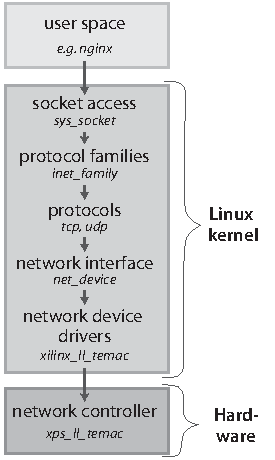
\includegraphics[scale=1]{images/net-stack.pdf}
	\caption{Linux network stack.}
	\label{fig:net-stack}
\end{wrapfigure}
The top most layer of the Linux network stack is the \textbf{system call interface} to create and operate on sockets \cite{netstackana}. The usage of this interface by \textit{nginx} is already described in section \ref{sec:nginx-os-if}. Its purpose is to multiplex networking calls by the user into the kernel \cite{netstackana}. Once a file descriptor was created using the socket interface, data can be exchanged with the network system through general operations on file descriptors like \textit{write} and \textit{read}, too. The socket interface is completely agnostic to different protocols or implementations by network devices and drivers. Its main underlying structure is "\texttt{struct sock}", containing all relevant information about a specific socket, like available functions and protocol specific state information.\footnote{\url{http://www.ecsl.cs.sunysb.edu/elibrary/linux/network/LinuxKernel.pdf}} Thereby also protocol and implementation specific functionality is bind to a socket using function pointers (defined in "\texttt{struct inet\_protosw}") \cite{netstackana}.

Whereas the more general data structure "\texttt{struct sock}" contains mainly meta information about a socket, the major structure for storing data is "\texttt{struct sk\_buff}". \textbf{\texttt{sk\_buff}} contains packet data and state information. It is used for to be sent, as well as for received packets almost through out all layers of the network stack. \cite{netstackana}

The gap between protocol handling and device drivers is bridged by the \textbf{network interface} (\textit{netif}) layer. This is a hardware device "agnostic interface layer" \cite{netstackana}. Its major purpose is to connect protocols to hardware devices. Information about devices is provided through "\texttt{struct net\_device}". On system start-up all available devices register themselves with a filled out "\texttt{net\_device}" structure. From there on they are know to the network interface layer.

The lowest layer of the network stack being part of the Linux kernel is formed by \textbf{device drivers}. These hook into the network interface layer and manage physical/hardware network controllers. For the implemented System on Chip this is the \texttt{xps\_ll\_temac} \gls{ip} core.

\begin{wrapfigure}[10]{r}{.23\textwidth}
	\centering
	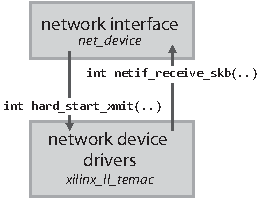
\includegraphics[scale=1]{images/netif-dev.pdf}
	\caption{\texttt{sk\_buff} exchange}
	\label{fig:netif-dev}
\end{wrapfigure}

Since introduction of the "New API" (\textit{NAPI}) for communication between device drivers processing packets and the network interface layer, most of the workload for received and to be sent packets is scheduled using software interrupt requests (also known as "\textit{soft irq}" or "\textit{sirq}").\footnote{\url{http://www.linuxfoundation.org/collaborate/workgroups/networking/napi} (as of 12/2012)} During performance tests described in the previous chapter this was visible through high CPU utilization of the \textit{sirq} category.

The network interface layer enqueues \texttt{sk\_buff} packets for transmission using the function \texttt{int hard\_start\_xmit(struct sk\_buff *skb, struct net\_device *dev)}. Usually a call to this function is protected with a \textit{lock} to protect it from being called multiple times simultaneously.\footnote{\url{http://lwn.net/Articles/120960/} (as of 12/2012)} The device driver pushes received packets to the upper layer using \texttt{int netif\_receive\_skb(struct sk\_buff *skb)}. \cite{netstackana}

\chapter{TCP Offload Engine}

\section{Overview}

\subsection{Benefits}

Conducted performance tests showed\footnote{see figures \ref{fig:initial-req-cpu} and \ref{fig:tcp-io-perf-cpu}} that much processing time is spend handling interrupt requests of the network sub system. Especially on TCP-heavy-requests this circumstance tuned out to be a bottleneck for a system with little processing power like the designed System on Chip.

Handling of TCP connections and processing messages is on the other hand a well defined and general problem that could be outsourced to an own "processor", leaving more processing power of the main system (\gls{cpu}) for other tasks. This is the approach of \textit{TCP Offload Engines} (TOE).
\\

\subsection{State of the Art}

Throughout recent years some attempts by hardware vendors developingBücher network interface cards were made to integrate support for \textit{TCP Offload Engines} into the Linux kernel (e.g. by \textit{Chelsio Communications}: \url{http://lwn.net/Articles/147289/}). However, maintainers\footnote{\url{http://lwn.net/Articles/148701/}} of the Linux network stack and the \textit{Linux Foundation}\footnote{\url{http://www.linuxfoundation.org/collaborate/workgroups/networking/toe}} have a strong opinion against integrating drivers and support through out the network stack for these hardware devices.

This is partially based on reservations about quality standards and the lack of possible benefits, but includes also arguments of a more general nature. A \textit{TOE} would "short out much of the Linux networking code" and therefore "cut out little features like \textit{netfilter}, traffic control, and more" \cite{linux-toe}. Additionally it is not easily possible to supply security fixes for \textit{TOE} functionality implemented in hardware. Therefore it would be necessary to cut off integration of a \textit{TOE} on occurring security vulnerabilities by releasing Linux kernel hot fix versions.

These are reasons why no support for \textit{TCP Offload Engines} is available in Linux kernel, currently. Of course all arguments are based on the point of view of Linux being a general purpose operating system used in desktop and server systems, powered by decent computer hardware. For embedded systems these assumptions are usually not fulfilled. Neither will the \textit{TOE} be part of an exchangeable and replaceable network interface card, supplied by a third-party vendor, but probably integrated into a System on Chip as an \gls{ip} core. Therefore the next sections will discuss approaches for an integration of dedicated engines, offloading TCP processing to hardware.
\\

\section{Possible Approaches}

There are a number of levels for offloading features to hardware. The simplest one is offloading checksum calculation to the network interface card. This is already implemented by the used \textit{xps\_ll\_temac} \gls{ip} core (see sec. \ref{preceeding:net}).
\\

\subsection{Large Segment and Receive Offload (LSO/LRO)}

Another option which is already supported by the network device layer of the Linux kernel is \textit{TCP Segmentation Offload} (TSO), also known as \textit{Large Segment Offload} (LSO).\footnote{\url{http://www.linuxfoundation.org/collaborate/workgroups/networking/tso} (as of 12/2012)} Inside of the Linux kernel, this technique uses very large data buffers in a single \texttt{sk\_buff} structure and therefore large \gls{tcp} packets far beyond typical \gls{mtu} values. Splitting these single packets to multiple packets of transmittable size (i.e. segmentation) is done by the network device, connected to the Linux kernel as a hardware device. This reduces the number of processed TCP packets and acknowledgments by the CPU, but leaves all state related tasks to the operating system. Therefore it prevents short cutting the network stack and additional functionality for network management and analysis. But it implicates known problems of transparent segmentation, too \cite{kn1}[sec. "5.5.7 Segmentation"].

The other way round is called \textit{Large Receive Offload} (LRO). This concept is supported by the \textit{New API} (NAPI) in Linux kernel for receiving network packets in the way that the number of hardware interrupt requests is reduced on high network utilization, but implemented completely in software \cite{linux-lro}.
\\

\subsubsection{TCP Chimney Offload}

Microsoft has introduced a technique called \textit{TCP Chimney Offload} with \textit{Microsoft\textsuperscript{\textregistered} Windows Server\textsuperscript{\textregistered} 2003 Scalable Networking Pack (SNP)}. This allows offloading the complete handling of TCP processing "on demand" to the network interface card. Connections are therefore known to the operating system and can be managed complete in software. But it is also possible to offload further processing of a connection to hardware to alleviate bottlenecks. Because not only packet, but also connection and state handling can be done by the hardware, the network interface card requires a complete implementation of the TCP/IP protocol stack. \cite{dell-toe}

This is a proprietary solution by Microsoft and some hardware vendors. There are no approaches of bringing it to the Linux kernel or other unix-based operating systems, to the knowledge of the author.
\\

\subsubsection{Full-stack TCP Offload}

The last to be introduced solution can be described as "\textit{Full-stack TCP Offload}". All processing of \gls{tcp} and \gls{ip} concerns is done by hardware. This requires a great deal of protocol knowledge and functionality to be implemented in hardware, but promises also the best performance gains, leaving just a minimal part of TCP/IP stack processing to the operating system.

This is the chosen way by the research project enclosing this thesis. Therefore the next section provides some considerations for integrating a \textit{TOE} following this concept into the Linux kernel and remarks concerning device driver development and interfaces of the \textit{TOE}.
\\

\section{Integration into Linux}

Integration of a \textit{Full-stack TOE} into the network stack of Linux kernel must consist of two major parts:

\begin{enumerate}
\item A network device driver handling communication with the actual \textit{TCP Offload Engine} device.
\item Changes to the current network stack for -- conditionally -- short cutting the existing TCP processing implementation.
\end{enumerate}

\textit{Chelsio Communications}, a hardware vendor, developing network interfaces, made an attempt to integrate an own \gls{toe} following this approach into the Linux kernel in 2005.\footnote{\url{http://lwn.net/Articles/147289/} (as of 12/2012)} Their solution called "\textit{OPEN TOE}" claimed to be vendor neutral and could therefore serve as a model for a custom implementation.\footnote{\url{http://lwn.net/Articles/146060/} (as of 12/2012)}

Central unit for communication with the \gls{toe} device is the new \texttt{struct toedev}. It represents "a new type of extended network device [\dots] with an additional set of methods" \cite{linux-toe}.

The provided additional methods are listed below:

\begin{verbatim}
int (*open)(struct toedev *dev);
int (*close)(struct toedev *dev);
int (*can_offload)(struct toedev *dev, struct sock *sk);
int (*connect)(struct toedev *dev, struct sock *sk);
int (*send)(struct toedev *dev, struct sk_buff *skb);
int (*recv)(struct toedev *dev, struct sk_buff **skb, int n);
int (*ctl)(struct toedev *dev, unsigned int req, void *data);
void (*neigh_update)(struct net_device *lldev,
		     struct toedev *dev,
		     struct neighbour *neigh, int fl);

Source: http://lwn.net/Articles/147289/
\end{verbatim}

The methods can easily mapped to known features of \gls{tcp}:

\texttt{open(..)}, respectively \texttt{connect(..)} for client scenarios, signals the availability for incoming TCP connections or initiates the creation of an outgoing TCP connection. \texttt{close(..)} ends an existing TCP connection.

The two functions \texttt{send(..)} and \texttt{recv(..)} are well known from the socket interface layer and facilitate transmission and receiving of single or multiple TCP packets in form of \texttt{sk\_buff} structures.

\texttt{can\_offload(..)} and \texttt{ctl(..)} provide control access to the TOE device. The function \texttt{neigh\_update(..)} is required for usage of the \textit{neighbor subsystem}\footnote{\url{http://www.linuxfoundation.org/collaborate/workgroups/networking/neighboringsubsystem} (as of 12/2012)} which enables discovery and mapping between physical (\textit{MAC}) and logical (\textit{IP}) network addresses.

The actual data in form of \texttt{sk\_buff} structures should be transferred to and from the TOE device using \gls{dma}. DMA stands for \textit{Direct Memory Access} and describes an architecture featuring direct memory access of devices to system's main memory. Therefore no processing power is deducted from the \gls{cpu} shifting data between the Linux kernel structures and the TOE device.

One challenge of \gls{dma} usage combined with a \gls{mmu} is the translation between virtual (used by the \gls{os}) and physical (used by the device) memory addresses. Continuous memory regions in virtual address space do not need to be continuous in physical address space. Therefore the device might be required to access multiple fragments of memory, although it was passed only a single data structure written by the Linux kernel.

DMA is on the other hand widely used for high bandwidth devices, which is why many references for these problems should exist, alleviating the implementation of appropriate solutions.

Without further knowledge about the concrete \gls{toe} implementation, this is as far as preparations and research on the topic of a possible integration into the Linux kernel can go. Next steps would be to work on that implementation.